
\label{chap: methods}
In this section, two methods are presented that attempt to reduce the bias seen in the estimates from \textcite{michelot_langevin_2019}. The first of these methods applies the EKF to an increased state-space model. The second is based on increasing the state space of the Langevin model using hidden states, then using the Monte Carlo method to integrate out the hidden states. 

\section{Extended Kalman Filter}
\textcite{kulikov_extended_2024} describes one method that tries to more accurately approximate the likelihood of diffusion processes using the EKF. If we use the EM method to describe a state-space model, we can then find a likelihood using the EKF. In addition, we can improve this likelihood approximation by adding extra hidden states between the states that we have observed. For the Langevin process, the state space representation is 

$$\textbf{X}_{k+1} = f(\textbf{X}_k) + \textbf{w}_k = \textbf{X}_k + \frac{\gamma^2\Delta_k}{2}\nabla \log(\pi(\textbf{X}_k)) + \textbf{w}_k,$$

$$\textbf{Z}_k = h(\textbf{X}_k) + \textbf{w}_k.$$

Where $\textbf{w}_k$ has a gaussian distribution with $0$ mean and covariance $\gamma^2\Delta_k I_{2*2}$, and $\textbf{v}_k$ has $0$ mean and covariance $\textbf{R}$. In the case where the process is being observed directly, the function $h$ is the identity function, and the matrix $\textbf{R}$ is a zero matrix. The method described in \textcite{kulikov_extended_2024} adds a mesh of $L$ hidden states to the state-space model between observations $\textbf{Z}_i$ and $\textbf{Z}_{i+1}$. When using the EKF on the added mesh states, only the predict step is performed since there are no observations. The likelihood is then computed using \eqref{eq: EKF likelihood}, which can be used to make estimates of the parameters. 

\

The matrices $\textbf{F}_k$ and $\textbf{H}_k$ in Section~\ref{sec: EKF} are the Jacobians of the transition and observation functions. Since the observation function $h$ is the identity function, we get $H_k = I_{2*2}$. Furthermore, we have $\textbf{F}_k = J(f) = J(\textbf{x} + \frac{\gamma^2 \Delta}{2}\nabla \log(\pi(\textbf{x}))) = I_{2*2} + \frac{\gamma^2 \Delta}{2} H(\log(\pi(\textbf{x})))$. $H(\log(\pi(\textbf{x})))$ is the Hessian of the log of the UD, which, if we insert the RSF, becomes $H(\sum_{i=1}^n \beta_i c_i(\textbf{x})) = \sum_{i=1}^n \beta_iH( c_i)(\textbf{x})$. The calculation of this matrix involves taking the second derivative of the covariate functions. This can be found using the method described in Subsection~\ref{subsec: second derivative}.




\section{Monte-Carlo Estimation of Likelihood}
\label{sec: Monte Carlo Estimation}
For the second method, consider a hidden variable $\textbf{Z} = (\textbf{Z}_1, \dots \textbf{Z}_n)$ that is a set of states between two observations of the Langevin process $\textbf{X}_k$ and $\textbf{X}_{k+1}$. We can write the joint density of transitioning from the first observation to the second observation via these states as 

$$p(\textbf{X}_{k+1}, \textbf{Z} | \textbf{X}_k) = p(\textbf{X}_{k+1}|\textbf{Z})p(\textbf{Z}|\textbf{X}_k) = q_{\Delta_k/(N+1)}(\textbf{X}_{k+1}|\textbf{Z}_N)\dots q_{\Delta_k/(N+1)}(\textbf{Z}_1|\textbf{X}_k).
$$ 

From here we can integrate out the hidden variable to get the likelihood of the observations, 


$$p(\textbf{X}_{k+1}|\textbf{X}_k) = \int q_{\Delta_k/(N+1)}(\textbf{X}_{k+1}|\textbf{Z}_N)\dots q_{\Delta_k/(N+1)}(\textbf{Z}_1|\textbf{X}_k)d\textbf{Z}.
$$

Because the time difference between the states in $\textbf{z}$, is smaller than the time difference between $\textbf{X}_{k+1}$ and $\textbf{X}_k$, so $q_{\Delta_k/(N+1)}$ should be a better approximation for the Langevin process than $q_{\Delta_k}$. We can approximate this integral by using the Monte Carlo method described in Subsection~\ref{sec: Monte Carlo integration}. We can sample M paths $\textbf{Z}^i = (\textbf{Z}_1^i, \dots,\textbf{Z}_N^i)$ each with N nodes, using $\textbf{Z}_{j+1}^i = \textbf{Z}_j^i + \nabla \log(\pi(\textbf{Z}_j^i)) + \frac{\Delta_k\gamma^2}{N+1}\bm \epsilon_j^i$ where $\bm \epsilon_j^i$ standard two-dimensional Gaussian distributions for $i=1, \dots , M$ and $j = 1,\dots , N$, using $\textbf{Z}_0^i = \textbf{X}_k$. We then get the likelihood estimate

$$
\hat{L}(\bm \beta , \gamma^2|X_k, X_{k+1}) =  \frac{1}{M}\sum_{i=1}^M q_{\Delta_k/(N+1)}(\textbf{X}_{k+1}|\textbf{Z}^i_N)\dots q_{\Delta_k/(N+1)}(\textbf{Z}^i_1|\textbf{X}_k).
\label{eq: montecarlo likelihood}
$$

If the hidden states $\textbf{Z}_i$ are evenly distributed in time, and the number of states $N$ is sufficiently high, then they should accurately approximate the Langevin process, as evidenced in Figure~\ref{fig:MALA}. In turn, this means the Monte Carlo likelihood estimate should be unbiased estimate for the transition likelihood of the Langevin process. An important point about this likelihood estimate is that it is stochastic, which has to be taken into account when maximizing the likelihood. 

\begin{comment}
\parencite{durham_numerical_2002} uses the Nelder-Mead optimization algorithm to find maximum likelihood estimates. This is a direct search method, meaning it does not compute the gradient of the function that is being minimized. This is an advantage when the likelihood estimate is stochastic since gradients require evaluating the function at close intervals which may be subject to a lot of noise.     
\end{comment}


\subsection{Importance Sampling}
\label{subsec: importance sampling}
One problem with the likelihood estimator \eqref{eq: montecarlo likelihood} is that the last step of the probability $q_{\Delta_k/(N+1)}(\textbf{X}_{k+1}|\textbf{Z}_N)$ often has a small value. This is because the paths $\textbf{Z}$ diverge more and more from the true path that the Langevin process used, which means that for many paths the last state ends far away from the next observation. In turn, this means that most simulations of $\textbf{z}$ contribute very little to the estimated likelihood, and a small number of simulations that end up landing close to $X_{k+1}$ end up contributing to a large part of the estimate, giving the estimate high variance. \textcite{durham_numerical_2002} improves upon the Monte-Carlo estimate of the transition by using importance sampling, described in Subsection~\ref{subsec: importance sampling}, into the method. Instead of sampling $\textbf{Z}$ from the Langevin process, they sample it from a different distribution $p$ and use the estimate

\begin{equation}
\hat{L}(\theta|X_k, X_{k+1}) = \frac{1}{M}\sum_{i=1}^M \frac{q_{\Delta_k/(N+1)}(\textbf{X}_{k+1}|\textbf{Z}^i_N)\dots q_{\Delta_k/(N+1)}(\textbf{Z}^i_1|\textbf{X}_k)}{p(\textbf{Z}_i)}.
\label{eq: importance sampling likelihood}
\end{equation}


\textcite{durham_numerical_2002} proposes a Brownian bridge between the observations $\textbf{X}_k$ and $\textbf{X}_{k+1}$ for the distribution $p$. This is a simulation of a Brownian motion $\gamma \textbf{B}_t$, conditioned on having endpoints $\textbf{X}_k$ and $\textbf{X}_{k+1}$. A Brownian bridge variable $\textbf{B}_l$ can be simulated as a multivariate Gaussian distribution with mean $\bm \mu_l = \textbf{X}_k + l(\textbf{X}_{k+1}-\textbf{X}_k)/N$ and covariance matrix $\bm \Sigma$ with $\bm \Sigma_{ij} = \bm \Sigma_{ji}= \Delta \gamma^2(1-\frac{i}{N+1}) \frac{j}{N+1}$ for $i = 1, \dots , N$ and $j = 1, \dots, i$. Here, N is the number of mesh nodes in the bridge. We can write the full log-likelihood as 


$$
\hat{l}(\bm \beta, \gamma^2) = \sum_{i = 1}^K \log( \frac{1}{M}\sum_{j=1}^M \frac{1}{P_{ij}}\prod_{k=0}^N \mathcal{N}(B_{ijk+1} ; B_{ijk+1} - \frac{\Delta \gamma^2}{2}, \Delta\gamma^2 I_{2*2})),
$$

where the first and last elements of the bridges $B_{ij0}$ and $B_{ijN+1}$ are the observed values of the Langevin process $X_i$ and $X_{i+1}$, respectively, and $P_{ij}$ is the density of the j-th bridge between $\textbf{X}_{i+1}$ and $\textbf{X}_i$.


To demonstrate how Brownian bridges reduce the variance of likelihood estimates, a Langevin process was simulated using a resolution of $0.01$ with the Perlin covariates from Figure~\ref{fig:covariate plots} and $\gamma^2 = 5$ up to time $0.1$. 10 Brownian bridges were then simulated using the same diffusion as the Langevin process, and 10 Langevin processes were simulated using the same setup as with the original Langevin process, but with the last increment of the process going to the endpoint of the original process. The results are shown in Figure~\ref{fig:monte carlo paths}. 


\begin{figure}[H]%
    \centering
    \subfloat[\centering Langevin process simulations]{{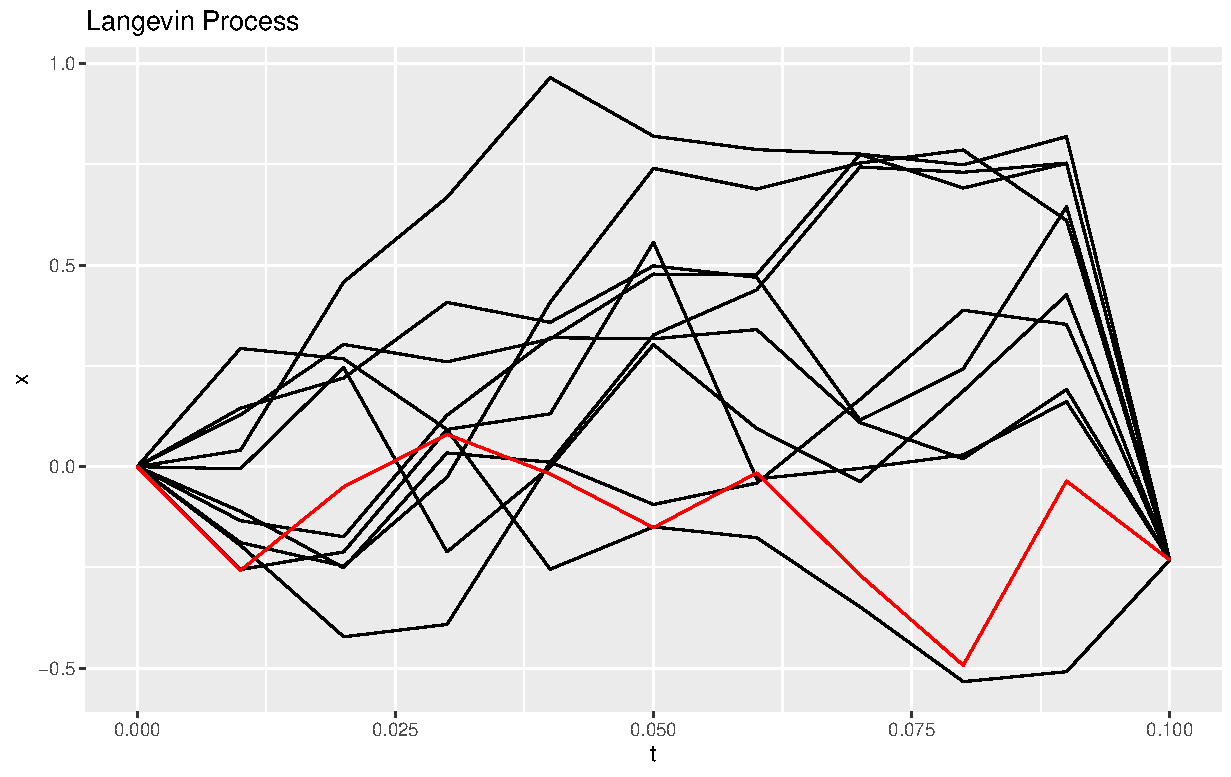
\includegraphics[width=\linewidth]{Images/methods/Langevin process path figure.pdf} }}%
    \qquad
    \subfloat[\centering Brownian bridge simulations]{{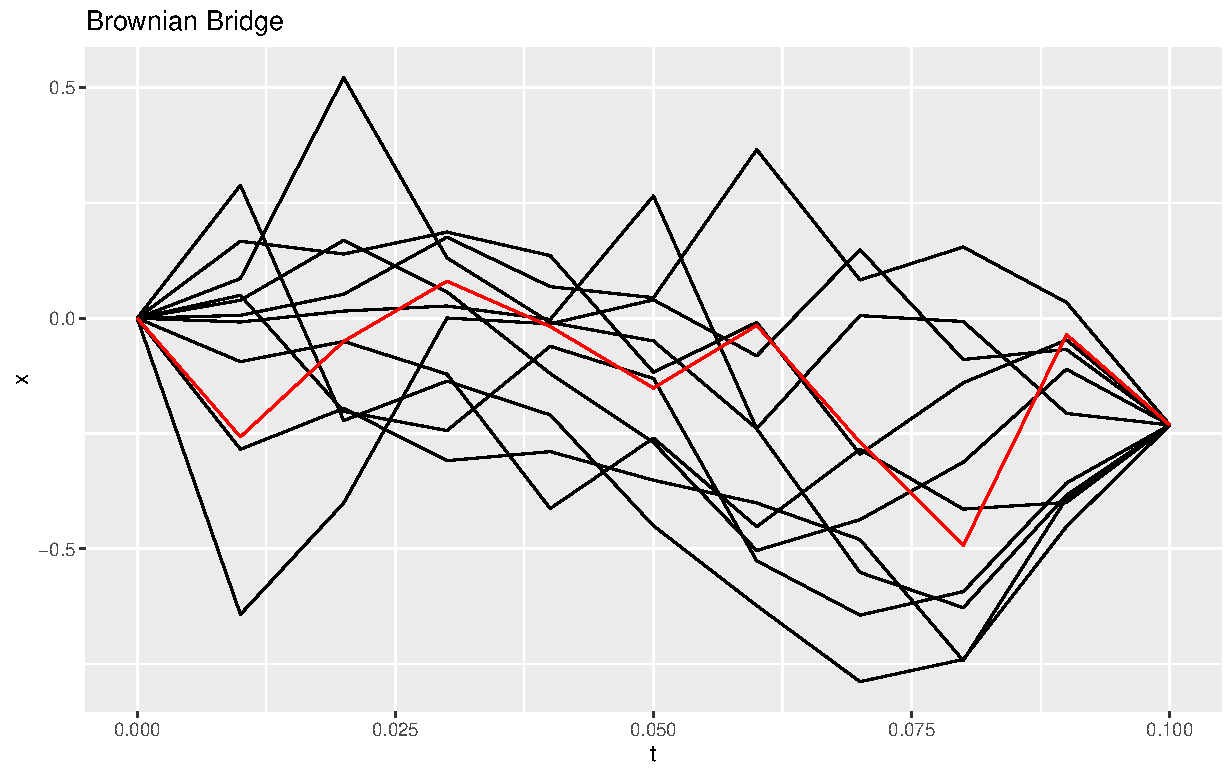
\includegraphics[width=\linewidth]{Images/methods/Brownian bridge path figure.pdf} }}%
    \caption[Langevin and Brownian bridge paths]{(a): 10 Langevin paths simulated at a resolution of $0.01$ using 10 steps in black. The last step is the path to the last position of the true path, shown in red. (b): Ten simulations of Brownian bridges with 10 nodes and endpoints at the end points of the Langevin process that we are estimating, shown in red.}%
    \label{fig:monte carlo paths}%
\end{figure}


The code for generating Figure~\ref{fig:monte carlo paths} can be found in the github repository in Appendix \ref{Appendix: github repo} under the file name "Langevin and Brownian bridge path figure". Figure~\ref{fig:monte carlo paths} shows one dimension of the paths simulated from the Langevin process in (a) and the Brownian bridge in (b), plotted against time. The true path of the Langevin process, whose endpoints we are simulating based on, is shown in red. The first figure shows how the final step of the simulated Langevin processes (black), in many cases, deviates from the Langevin process that we are trying to estimate. Since there is high variability in the distance from the last point in $\textbf{Z}^i$ to the next observation, this can cause the likelihood estimate to have a high variance. The second plot, on the other hand, shows that the proposed paths do not include large jumps, as the first plot. Because of this, using the Brownian bridges as a proposal density might reduce the variance of the likelihood estimate. judging by the Langevin process in red, the Brownian bridges are also plausible transitions of the Langevin process. 


Using the theory of subsection~\ref{subsec: importance sampling theory}, the density of the variables being integrated with respect to $f(x)$, is the EM transition probability. The density of the proposal, $g(x)$, is the probability of the Brownian bridge, and the function we are integrating over$h(x)$, is the probability transitioning in the last step to the end points of the Langevin process $q_{\Delta_k/(N+1)}(\textbf{X}_{k+1}|\textbf{Z}_N)$. The support of $f$ is the same as the support of $g$, since both the Langevin process and the Brownian bridge can theoretically take on any value for any of the mesh states. When $g$ is small, $h$ is also likely to be small, indicating that the Brownian bridge should reduce the variance. \textcite{durham_numerical_2002}  shows that the importance sampling estimator reduces the root mean square error to the Langevin process, compared to using the Monte Carlo estimate.


\subsection{Precomputing Brownian Bridges}
\label{subsec: precomputing brownian bridges}
Even when using importance sampling, it can take a long time to compute the likelihood. A large portion of the computational complexity of the likelihood is simulating the Brownian bridges and computing the gradients of the covariates at the points of the bridges. A way to circumvent some of this computation would be to simulate the bridges and compute the gradients before evaluating the likelihood. This might save time in situations where we are evaluating the likelihood many times, like in numerical optimization. Precomputing the Brownian bridges would necessitate having a value for the speed parameter beforehand. One way of doing this is to use the estimate from \textcite{michelot_langevin_2019} for the speed parameter. For large time differences between observations, this estimator underestimates the speed. However, if the variance used in the proposal has little effect on the likelihood estimate, this could still give the correct parameter estimates. 













